\chapter{Mise en œuvre}
\section{La demande du client}

 \section{La gestion de projet}

  \subsection{Communication au sein du groupe}

    Dans un projet de cette importance et mené par autant de personnes, une
    bonne communication est essentielle afin d'éviter des situations où des
    membres d'une équipe ne se comprennent pas.

    Pour garantir cette bonne communication, nous avons donc organisé des
    réunions toutes les 2 semaines afin de maintenir une même vision du projet,
    la circulation de certaines informations, ainsi que la cohésion de l'équipe
    .

    Le groupe étant divisé en plusieurs équipes, des réunions d'équipe ont
    également lieu afin de pouvoir réaliser la tâche qui leur a été attribuée
    dans les meilleures conditions.

    Des systèmes d'échanges d'informations ont aussi été mis en place, comme le
    système de tickets (sur le site GitHub), afin de résoudre au plus vite tout
    problème faisant obstacle à l'un des développeur.

    De plus, la communication au sein de notre groupe nous a permis de définir
    clairement le rôle de chacun.


  \subsection{Méthodologie employée}

    Le développement de ce projet s'est fait selon la méthode \emph{eXtreme
    Programming}. Cette méthode a aidé les membres du groupe à travailler de
    façon cohérente les uns par rapport aux autres.

    Un des principes fondamentaux de la méthode \emph{eXtreme Programming} est
    d'établir des tests de façon systématique (\emph{Test Driven Development}),
    ce qui amoindri le nombre d'erreurs à la fin de chaque étapes du
    développement. De plus on voit clairement, une fois les tests établis, à
    quelles exigences la fonctionnalité développée doit répondre : cela rend
    plus simple le développement.

    La méthode XP s'intégrait très bien à nôtre projet, puisque ses principales
    valeurs sont :
    \begin{description}
      \item[La communication :] Faire en sorte que tous aient une bonne vision
      du projet, des ses objectifs, de son avancement et de ce qu'ils doivent
      faire, y compris les personnes extérieures au projet.
      \item[Le feed-back :] Le projet doit aussi être régulièrement contrôlé
      afin de ne pas dévier du but initial fixé par le client. Les tests
      unitaires constituaient un retour d'information efficace côté
      développement pour s'assurer du bon fonctionnement du code. Et les
      réunions et livraisons régulières auprès du client permettent de
      témoigner de l'avancement global du projet.
      \item[La simplicité :] La solution la plus simple est toujours la
      meilleure et la plus facile à faire évoluer.
    \end{description}


  \subsection{Suivie du projet}

    Une bonne cohésion du groupe est essentielle (comme vu plus haut), mais
    nous devons aussi établir une communication solide avec le client afin de
    répondre correctement à ses attentes.

    Des réunions régulières avec les clients, qui ont eu lieu à peu près toutes
    les 2 semaines, ont permis de faire évoluer le projet de façon conforme,
    c'est-à-dire en accord avec les besoins des clients, tout au long du projet
    .

    Le suivis était, pour la plus grande partie réalisé par la maîtrise
    d'ouvrage, qui tenait le reste de l'équipe informée, gardant ainsi un lien
    bien établi avec le client.


  \subsection{Les documents de gestion de projet}

    Dans un projet, les documents de gestion de projet font office de feuille
    de route. Ils définissent les objectifs, le cadre, les ressources humaines
    et les ressources en temps.

    La délimitation des tâches à effectuer est donc formalisée par les
    différents documents de gestion de projet, ce qui nous permet un découpage
    efficace du développement du projet et donc d'avancer plus rapidement.

    Le diagramme de Gantt est un autre type de document d'une grande aide sur
    un projet d'une telle envergure : on y voit clairement la situation de
    chacun par rapport au projet, les tâches en cours, les ressources, etc.
    L'avancement du projet y apparait aussi clairement de même que toutes les
    dates importantes. C'est un document à mettre à jour très régulièrement.

    \href{../graphics/gantt2-0.png}{capture}

    Les documents ont donc été particulièrement utiles notamment, l'\emph{
    analyse des risques} dont le formalisme a rendu la résolutions d'obstacle
    plus simples. D'une manière plus générale, ils nous ont guidé à travers ce
    projet conséquent en nous évitant d'être confronté à des problèmes pour
    lesquels aucune solution n'était encore en place, ils nous ont aussi évité
    de possibles déroutes.

  \subsection{Le rôle de chacun}

    La définition précise du rôle de chacun permet de définir des
    interlocuteurs pour chaque situation. De même cela évite qu'un problème
    soit pris en charge par plusieurs personnes.

    La composition du groupe est la suivante :
    \begin{itemize}
      \item Le chef d'équipe : Adrien \bsc{Smondack} (chef adjoint : Gaëtan
      \bsc{Ferry})
      \item La maîtrise d'ouvrage : Benjamin \bsc{Zigh} et Maxime \bsc{Michotte
      }
      \item Le responsable qualité : Gaëtan \bsc{Ferry} et Claire \bsc{Hardouin
      }
      \item Les responsables techniques : Damien \bsc{Picard} (C) Yves \bsc{
      Adegoloye} (Java Android)
    \end{itemize}


  \subsection{Conclusion}

    Tout au long du projet les méthodes employées ont permis une meilleure
    coordination au sein de l'équipe, et d'assurer une qualité de rendu
    optimale.

    Cette approche méthodique a été bénéfique à tous les niveaux du projet (
    communication, prévision, développement, etc). Elle définit un cadre
    nécessaire à l'accomplissement du projet en fixant des exigences en terme
    de qualité et de contenu des livrables.


\newpage
%------------------------------------------------------------------------------
\section{Le Module PAM}
\subsection{Pourquoi un module PAM ?}
La première solution d'implémentation envisagée était de reprogrammer un
serveur d'authentification complet. Cette solution posait deux problème:
\begin{enumerate}
  \item L'implémentation d'un protocole de communication.
  \item Inutilisable pour d'autres services en l'état.
\end{enumerate}

L'implémentation d'un module PAM résout ces deux problèmes, il est utilisable
par de nombreux services et le protocole de communication est du ressort du
service qui va utiliser le module. Cela a eu pour conséquence de réduire le
temps de développement et d'augmenter les possibilité offertes.

\subsection{Programmation de bibliothèques utilitaires}
Avant de débuter la programmation du module PAM il était nécessaire de créer
quelques bibliothèques utilitaires. Nombre d'entre elles permettront
d'abstraire la gestion de la mémoire et d'offrir une vision de plus haut niveau
du langage. De plus cet étape permettait un travail collaboratif simplifié.

La méthodologie pour le développement était la suivante:
\begin{itemize}
  \item Rédaction des fichiers d'en-tête contenant les prototypes et la
  documentation des fonctions à implémenter.
  \item Rédaction des éventuels test unitaires.
  \item Implémentation des fonctions.
  \item Exécution des tests, en cas d'échec retour à l'étape développement.
\end{itemize}

\subsubsection{Bibliothèque de gestion de secret}
Cette bibliothèque est chargée de gérer la représentation de secrets en mémoire.
Un secret est une suite d'octet partagée avec le token. Celui ci peut être
représentée comme une suite de caractères \verb?ASCII? ou hexadécimale.

Dans cette bibliothèque nous trouverons:
\begin{itemize}
  \item une structure \verb?secret?, qui consiste en un pointeur sur un tableau
  d'octets et une longueur codée sur un entier.
  \item Des fonctions de création chargée d'allouer l'espace mémoire requis en
  fonction du nombre d'octets désirés ou d'une entrée utilisateur.
  \item Des fonction chargé de représenter un secret dans différentes bases
  sous la forme de chaînes de caractères.
  \item Une fonction permettant d'effacer un secret de la mémoire et de
  libérer les ressources.
\end{itemize}

\subsubsection{Bibliothèque de calcul de mot de passe jetable}
Cette bibliothèque est chargé d'implémenter l'algorithme de génération de mot
passe jetable tel que décrit dans la RFC 4226\cite{HOTPrfc}. Elle ne fourni
qu'une fonction de génération. Pour générer un HOTP on lui passera un compteur
arbitraire. Pour générer un TOTP on lui passera le temps en tant que compteur.

\subsubsection{Bibliothèque de gestion des utilisateurs}
Cette bibliothèque est chargé d'abstraire la gestion des utilisateur, ces
derniers ainsi que leurs informations sont enregistrés dans un fichier texte
brut.

Nous nous sommes donc dotés des outils suivants:
\begin{itemize}
  \item Une structure en mémoire représentant un utilisateur et ses
  informations.
  \item Une fonction d'enregistrement d'une structure dans le fichier.
  \item Une fonction permettant d'obtenir une structure utilisateur du fichier
  à partir d'un nom d'utilisateur.
  \item Deux fonctions pour poser et libérer un verrou sur le fichier.
  \item Une fonction permettant de gérer les ressources mémoires.\\
\end{itemize}

Les fonctions de gestion de verrouillage sont la pour gérer les accès concurrents
au fichier des utilisateurs. Il faut prévoir que ces fonction seront appelées
dans un module chargé par différent service. Et donc sans ce verrou il devenait
impossible de garantir qu'un OTP ne puisse pas être utilisé deux fois, Si deux
processus lisent les information au même moment et permette l'authentification
alors un OTP fonctionnera plusieurs fois.

\subsubsection{Bibliothèque de gestion des options}
Cette bibliothèque permet de gérer les options fournies au module lors du chargement
par le service. Cela permet d'adapter un comportement différent pour chaque option fournie.\\
Dans cette bibliothèque nous trouverons:
\begin{itemize}
  \item Une structure \verb?modopt?, qui contient la valeur ou l'état de chaque option.
  \item Une fonction qui rempli la structure précédente d'après le contenu fourni en paramètre.
  \item Une fonction qui modifie la valeur ou état de l'option souhaité.
  \item Une fonction qui renvoie la valeur ou l'état d'une option.
\end{itemize}

\subsection{Programmation avec PAM}
\subsubsection{Fonction d'authentification}
Cette fonction permet d'authentifier un utilisateur. Chaque service configuré
pour utiliser le module exécutera cette fonction. Elle implémentera les
mécaniques de vérification telles que décrites dans les RFC ainsi que les
mécaniques de resynchronisation.
\paragraph{HOTP}
Pour HOTP la vérification de l'otp courant correspondant au compteur
$n$\footnote{Strictement positif.\label{int}} la vérification s'effectuera sur
une fenêtre de  $k$ $^{\ref{int}}$ otp, c'est à dire qu'elle va comparer l'otp
fourni aux otp de compteur $n$ à $n+k$ inclus. En cas de succès on enregistrera
le compteur courant comme nouveau compteur, c'est la phase de resynchronisation.
\paragraph{TOTP}
Pour TOTP la vérification de l'otp courant correspondant à un temps $t$ avec un
quantum $q$ se fera sur les otp $\frac{t}{q} - 2$ à $\frac{t}{q} + 2$ avec un
pas de $1$.
\paragraph{Problème d'attaque exhaustive}
On peut considérer qu'un OTP est une suite de 6 à 8 chiffres. Il est donc aisé
de tous les générer en moins de 30 secondes, pour preuve le rapport de test
indique 52ms pour 100 otp sur un smartphone android d'entrée de gamme,
il faut donc de 8m40s à 14h26m40s pour les générer sur un smartphone de faible
puissance. Sur une machine standard \footnote{Processeur: i5-3210M, RAM: 8Go} ce
n'est l'affaire que d'une dizaine de secondes.

Dès lors on voit la possibilité d'exécuter une attaque exhaustive réussie contre
le module devenir un problème bien réel. Pour palier à ce problème une première
solution était de bannir un utilisateur après un nombre fini d'essai raté. Après
discussion avec le client la solution retenue est un bannissement limité. Cela
consiste a rejeté toute tentative d'authentification pendant un laps de temps
après une tentative ratée.

Le delai par défaut est d'une secondes, on peut le modifier à l'aide des options
\verb?delay_totp? et \verb?delay_hotp? au chargement du module\footnote{voir le
Manuel d'installation du module PAM pour plus d'information}.

Avec ce nouveau paramètre, pour HOTP, il faut donc $\frac{p\times10^{l}*d}{w}$
secondes pour avoir $p\times100\%$ de chance de réussite avec des otp de
longueur $l$ et une fenêtre de $w$ dans un delai de $d$.

Pour TOTP cela revient même à réduire les chance de réussite d'une attaque
exhaustive à une probabilité de $\frac{q\times w}{d\times10^{l}}$ avec des OTP
sur un quantum $q$, d'une longueur $l$ avec un delay $d$.

%-------------------------------------------------------------------------------
\subsubsection{Fonction d'initialisation de secret}
Cette fonction permet d'implémenter la demande d'initialisation de secret.
C'est cette fonction qui sera appelé lorsqu'un service configuré pour utiliser
le module fera une demande de renouvellement de secret. Cette fonction demandera
à l'utilisateur de s'authentifier si c'est possible puis demandera les nouvelles
information d'authentification, c'est à dire:
\begin{itemize}
  \item La méthode d'authentification.\hfill\textbf{totp ou hotp}
  \item Le quantum si la méthode est totp.\hfill \textbf{un entier positif}
  \item La longueur des otp générés.
  \hfill\textbf{entiers compris entre 6 et 8 inclus}
\end{itemize}
Une fois ces information fourni le secret sera affiché. Cela implique que le
renouvellement de secret doit se faire lorsque la connexion est sûre.

%-------------------------------------------------------------------------------
\newpage
%------------------------------------------------------------------------------
\section{L'application Android}
Dans toute cette partie, ce qui sera appelé \emph{token}, sera en fait un triplet clef secrète, 
compteur, nom pour HOTP et un couple clef secrète, nom pour TOTP. C'est en fait un abus de notation
puisque le nom \emph{token} représente en fait l'unité matérielle (le terminal mobile) ou logicielle
(l'application) de génération de mots de passe.

\subsection{La bibliothèque de calcul}
Afin que le token soit en mesure de générer des mots de passe jetables, il était
nécessaire de développer une suite de fonctions de calcul. De plus, ces fonctions devait
être cohérentes avec celle écrites pour la vérification dans le module PAM.

La bibliothèque est découpée en trois partie distinctes tel que décrites sur la figure
\ref{fig:umlLib}. On trouve donc un ensemble de quatre classes formant la partie calcul
des mots de passe jetables, un deuxième de deux classes formant une couche d'abstraction
pour la gestion des secrets cryptographiques et enfin une dernière classe utilitaire
contenant des fonctions nécessaires aux protocoles HOTP et TOTP.

\begin{figure}
  \centering
  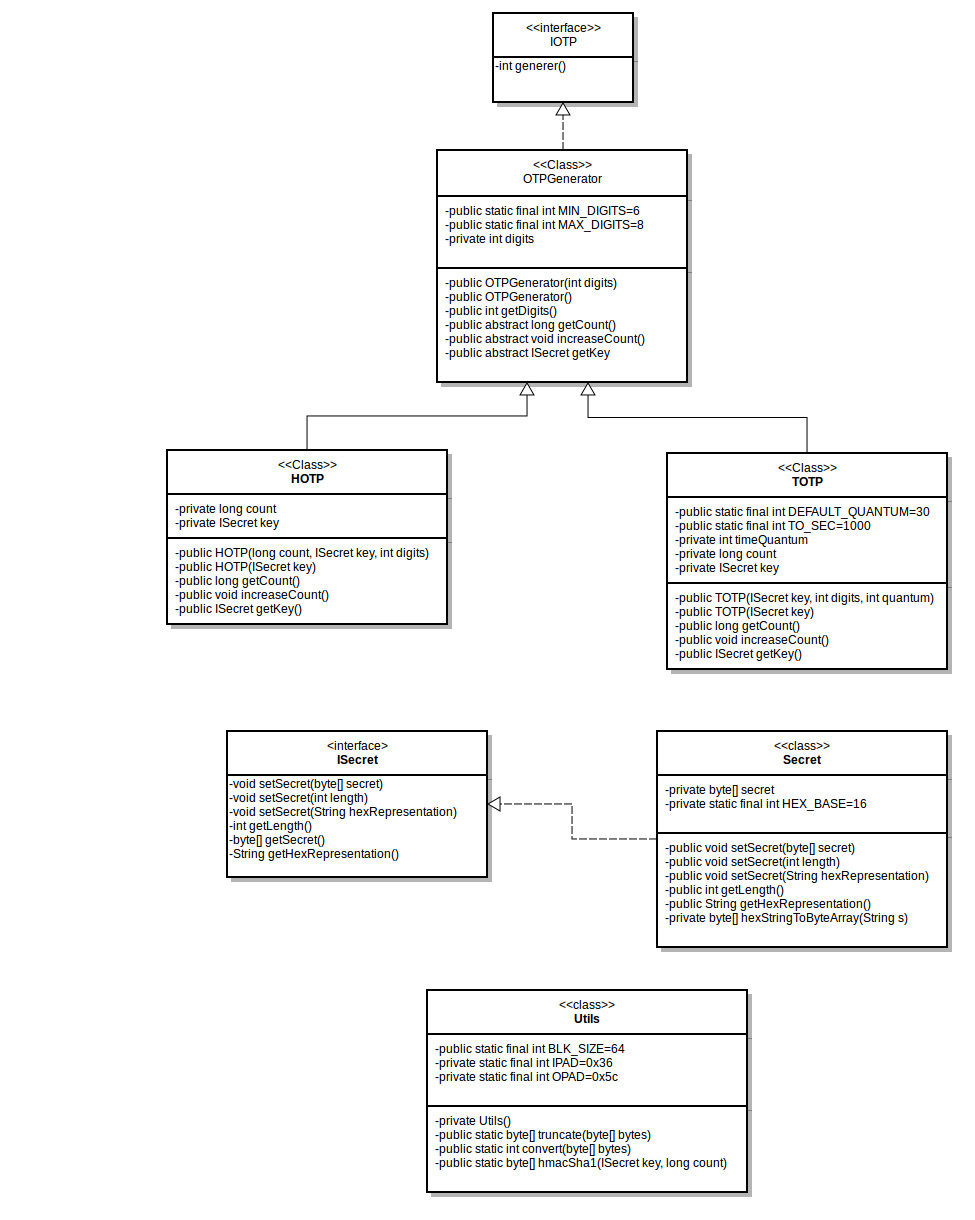
\includegraphics[scale=0.4]{../graphics/uml_lib.jpg}
  \caption{Architecture de la bibliothèque de calcul}
  \label{fig:umlLib}
\end{figure}

\subsubsection{Générateur d'OTP}
La première des trois partie définit les générateur d'OTP en eux même. Il sont répartis en
deux catégorie, correspondant aux deux méthode de génération implémentées, les générateur
TOTP et les générateur HOTP. Du fait que la spécification du protocole TOTP découle de celle
de celui d'HOTP, ces deux types d'objet sont très similaire dans leur fonctionnement. Les
parties communes des deux classes sont donc factorisées dans une classe abstraite. On
retrouve donc explicitées dans cette classe les méthodes pour récupérer le nombre de chiffre
composant les OTP ainsi que celle pour générer ces derniers. En effet, il est possible de
déclarer cette méthode à cette endroit en déportant la récupération du paramètre "compteur"
dans les classes inférieures. De ce fait, chacune des classes HOTP et TOTP défini sa
méthode \emph{getCounter} qui dans un cas retournera l'incrément du compteur synchronisé et
dans l'autre la valeur $ timestamp / quantum $ définie dans la rfc 4226\cite{TOTP}.

Le fonctionnement général des générateurs d'OTP est définit dans l'interface de
programmation IOTP. Cette interface reprend globalement le contenu des rfc 4226 et 6238.

\subsubsection{Gestion des secrets utilisateurs}
La deuxième partie formant l'abstraction des secrets cryptographiques est composée d'une
interface de programmation, \emph{ISecret}, et d'une classe l'implémentant, \emph{Secret}.
Elle a pour but de fournir une couche d'abstraction pour simplifier l'utilisation des secrets
qui peut s'avérer inconfortable dès lors que ces derniers mesures plusieurs dizaines de
caractère hexadécimaux.

On pourra donc grâce à ces deux classe créer des secrets pouvant être initialisés depuis des
données binaires brutes, des représentations hexadécimales ou encore depuis des données
aléatoires. De la même manière, il sera possible de récupérer un secret sous représentation
binaire ou sous la forme d'une chaine de caractère hexadécimaux.

\subsubsection{Fonctions utilitaires}
Enfin la dernière partie de la bibliothèque de calcul déclare des fonctions utilitaires
nécessaires aux calculs des mots de passes jetables. Concrètement, on y retrouve la
définition de la fonction HMAC\cite{HMACrfc} ainsi que des deux algorithmes de troncature et
de conversion définis dans la rfc 4226.

L'ensemble de ces fonctions est utilisé dans la classe abstraite \emph{OTPGenerator} pour la
génération des mots de passe jetables.

%--------------------------------------------------------------------------------
\subsection{Architecture de l'application}

L'application est architecturée autour de six écrans principaux représentant chacune une 
action réalisable par l'utilisateur. 

\subsubsection{Splash screen}
La première phase de l'application constituée par l'écran de \emph{splash screen} n'est pas à 
proprement parler un outil pour l'utilisateur. Elle permet en fait de charger les données enregistrées
de l'utilisateur dans la mémoire de l'appareil. Dans le même temps, elle tente de contacter un serveur
de temps NTP pour obtenir la valeur du décalage entre le temps système de l'appareil et le temps réseau
exacte. Cette valeur est alors stockée avec les autres données de l'utilisateur et cet écran passe la
main à celui de connexion (ou de création de PIN en cas de première connexion).

\subsubsection{Écran de PIN}
Il existe deux écrans relatifs aux entrées de PIN de l'utilisateur. Le premier permet la création
du PIN, et donc l'enregistrement de ce dernier dans le fichier local approprié. Le second permet
simplement la connexion de l'utilisateur et le déverrouillage de l'application\ref{secu}. Ces deux
écrans dirigent l'utilisateur vers l'écran de listing des \emph{tokens} ou vers celui de création 
si aucun n'existe.

\subsubsection{Ajout de token}
La page d'ajout de token permet à l'utilisateur d'ajouter ses différents \emph{tokens} de
génération. On peut y créer différents générateurs de mots de passe jetable en fournissant la 
méthode à utiliser (HOTP ou TOTP), la clef secrète à utiliser, la longueur des mots de passe à
générer et, si la méthode utilisée est TOTP, la durée de validité des mots de passe générés. Les 
générateurs ainsi créés sont alors disponibles dans la liste des tokens de l'utilisateur et 
directement utilisables. La terminaison de cet écran amène celui de visualisation de tokens
disponibles.

\subsubsection{Liste des tokens utilisateurs}
La page de listing des \emph{tokens} est centrale dans l'application. En effet, si il est impossible sur
celle ci d'effectuer d'autres opérations que la suppression de \emph{token}, c'est par elle qui faut 
passer pour joindre toutes les autres pages en utilisant le menu. Ce dernier permet d'accéder aux page
de suppression et d'ajout de token, et à celle de modification de code PIN. C'est aussi de puis ce
dernier que l'on peut accéder à la fonction de resynchronisation d'horloge (qui interroge des serveurs
ntp de la même manière que pendant l'écran de \emph{splash}).

C'est aussi depuis la liste des \emph{tokens} existants que l'on peut demander à l'un de ces derniers 
de générer son mot de passe jetable actuel.

\subsubsection{Suppression des tokens}
La page de suppression des \emph{tokens} n'est pas primordiale puisque sa fonction est redondante avec
la suppression de la page de listing.

\begin{figure}
  \centering
  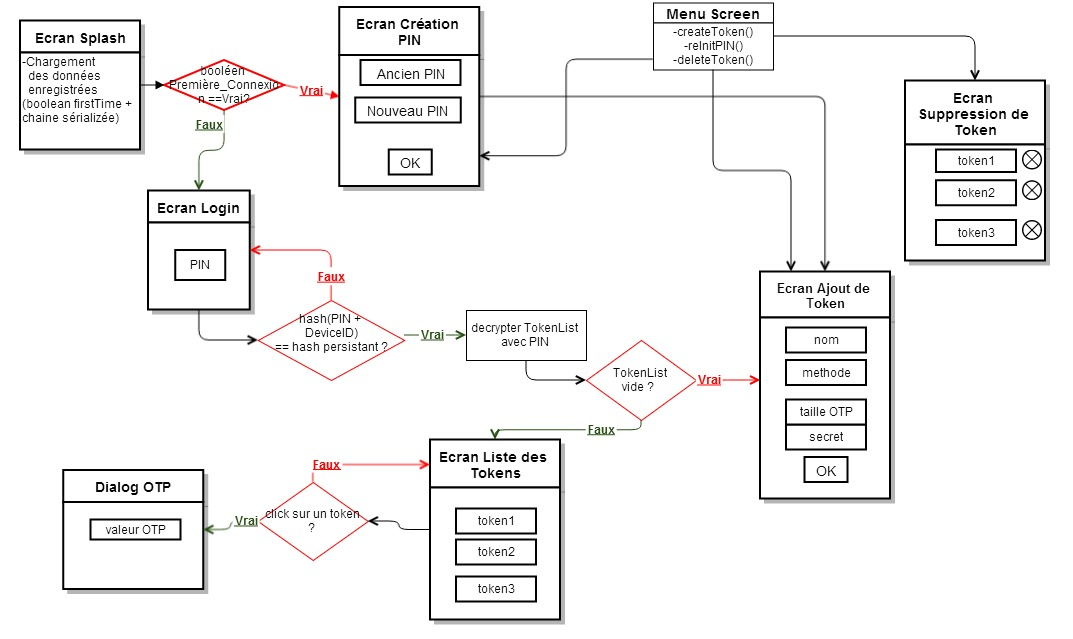
\includegraphics[scale=0.4]{../graphics/archi-android.jpg}
  \caption{Architecture de la bibliothèque de calcul}
  \label{fig:umlLib}
\end{figure}

\subsection{Sécurisation}
\label{secu}
La sécurisation de l'application est essentielle à la sécurité de l'ensemble du projet. En
effet, c'est elle qui va garantir que l'authentification mise en place est bien une
"authentification forte" grâce à l'ajout d'un facteur supplémentaire. L'enjeu de cette
partie est de garantir les 3 points suivant :


\begin{itemize}
  \item[1 -] Un utilisateur honnête doit pouvoir déverrouiller l'application en utilisant
  sont PIN. Il doit ensuite être en mesure de générer des mots de passe jetable en utilisant
  un de ses \emph{tokens} ou utiliser n'importe quelle autre fonctionnalités à sa
  disposition.
  \item[2 -] Un attaquant qui ne connaitrait pas le PIN de l'utilisateur ne doit pas être en
  mesure de déverrouiller l'application et donc de générer des mots de passes jetables en
  utilisant les \emph{tokens} de l'utilisateur.
  \item[3 -] Un attaquant qui ne connaitrait pas le PIN de l'utilisateur ne doit pas être en
  mesure, en parcourant le système de fichier de l'appareil, d'obtenir les clefs secrètes
  de génération.
\end{itemize}

La solution retenue consiste en la mise en place d'un PIN de déverrouillage de l'application.
Ce PIN, demandé à chaque démarrage de l'application, sera dans un premier temps haché par la
fonction SHA-1 en utilisant comme sel le \emph{device id} de l'appareil hôte. L'empreinte
obtenue est alors comparée avec celle enregistrée lors de la création du PIN dans un fichier
local. Si les deux valeurs sont cohérente, le PIN est alors utilisé pour déchiffrer le
fichier local contenant les informations relatives aux différents \emph{tokens} de
l'utilisateur. L'application devient alors pleinement utilisable.

Afin d'assurer une sécurité optimale des clefs de l'utilisateur, le chiffrement utilisé pour
le fichier local des \emph{tokens} est AES-256. Ainsi, on garantit que même après accès au
fichier sensible de l'application, un attaquant ne pourra virtuellement jamais accéder aux
clefs secrètes qui y sont stockés. De la même manière, le fait que le PIN de déverrouillage
soit stocké sous la forme d'un haché, implique que même après accès au fichier de stockage du
PIN, l'attaquant ne pourra pas déduire le PIN de l'utilisateur et donc la clef AES de
déchiffrement du fichier de \emph{token}. Il est à noter que le fichier contenant les données
privées de l'utilisateur n'est jamais déchiffré autre-part qu'en mémoire. Ainsi, même pendant
que l'application est déverrouillée et en court d'utilisation un attaquant ne pourra pas lire
le fichier en question. De la même manière, les informations ne seront pas accessible si 
l'application \emph{crash} en cours d'utilisation.




